%
% "The UCD CASL SenseTile System", for IEEE Pervasive Computing Joseph
% R. Kiniry, Vieri del Bianco, Dragan Stosic $Id: paper.tex 2795
% 2007-09-23 19:35:53Z dmz
%

\documentclass{article} \usepackage{times}

\usepackage{ifpdf} \usepackage{a4wide} \usepackage{pdfsync}

\ifpdf \usepackage[pdftex]{graphicx} \else \usepackage{graphicx} \fi

\usepackage{xspace} \usepackage{tabularx} \usepackage{epsfig}
\usepackage{amsmath} \usepackage{amsfonts} \usepackage{amssymb}
\usepackage{eucal} \usepackage{stmaryrd} \usepackage{float}
\usepackage{listings} % @(#)$Id: jml-listings.tex,v 1.6 2007/06/25 22:37:23 leavens Exp $
%
% Copyright (C) 2006 Iowa State University
%
% This file is part of JML
%
% JML is free software; you can redistribute it and/or modify
% it under the terms of the GNU General Public License as published by
% the Free Software Foundation; either version 2, or (at your option)
% any later version.
%
% JML is distributed in the hope that it will be useful,
% but WITHOUT ANY WARRANTY; without even the implied warranty of
% MERCHANTABILITY or FITNESS FOR A PARTICULAR PURPOSE.  See the
% GNU General Public License for more details.
%
% You should have received a copy of the GNU General Public License
% along with JML; see the file COPYING.  If not, write to
% the Free Software Foundation, 675 Mass Ave, Cambridge, MA 02139, USA.
%
% A JML listings environment.
%
% AUTHOR: Gary T. Leavens
%
% requires listings i.e., do \usepackage{listings} first
%
% This file is set up to be used via % @(#)$Id: jml-listings.tex,v 1.6 2007/06/25 22:37:23 leavens Exp $
%
% Copyright (C) 2006 Iowa State University
%
% This file is part of JML
%
% JML is free software; you can redistribute it and/or modify
% it under the terms of the GNU General Public License as published by
% the Free Software Foundation; either version 2, or (at your option)
% any later version.
%
% JML is distributed in the hope that it will be useful,
% but WITHOUT ANY WARRANTY; without even the implied warranty of
% MERCHANTABILITY or FITNESS FOR A PARTICULAR PURPOSE.  See the
% GNU General Public License for more details.
%
% You should have received a copy of the GNU General Public License
% along with JML; see the file COPYING.  If not, write to
% the Free Software Foundation, 675 Mass Ave, Cambridge, MA 02139, USA.
%
% A JML listings environment.
%
% AUTHOR: Gary T. Leavens
%
% requires listings i.e., do \usepackage{listings} first
%
% This file is set up to be used via % @(#)$Id: jml-listings.tex,v 1.6 2007/06/25 22:37:23 leavens Exp $
%
% Copyright (C) 2006 Iowa State University
%
% This file is part of JML
%
% JML is free software; you can redistribute it and/or modify
% it under the terms of the GNU General Public License as published by
% the Free Software Foundation; either version 2, or (at your option)
% any later version.
%
% JML is distributed in the hope that it will be useful,
% but WITHOUT ANY WARRANTY; without even the implied warranty of
% MERCHANTABILITY or FITNESS FOR A PARTICULAR PURPOSE.  See the
% GNU General Public License for more details.
%
% You should have received a copy of the GNU General Public License
% along with JML; see the file COPYING.  If not, write to
% the Free Software Foundation, 675 Mass Ave, Cambridge, MA 02139, USA.
%
% A JML listings environment.
%
% AUTHOR: Gary T. Leavens
%
% requires listings i.e., do \usepackage{listings} first
%
% This file is set up to be used via \input{jml-listings}.
% If you want, you could make a version that is a style file,
% but then change \lstdefinelanguage to \lst@definelanguage below.
%
\lstdefinelanguage[JML]{Java}[]{Java}%
       {% C++ style comments have to start with a blank!
        comment=[l]{//\ },
        % And C-style comments must also start with a blank or star!
        morecomment=[s]{/*\ }{*/},        
        morecomment=[s]{/**}{*/},
        % sensitive=true, % inherited
        % Add JML keywords as level 1 keywords, so can typeset differently
        classoffset=1,
        % And here are all the wonderful JML keywords
        morekeywords={abrupt_behavior,abrupt_behaviour,
         accessible,accessible_redundantly,also,assert,assert_redundantly,
         assignable,assignable_redundantly,assume,assume_redundantly,
         axiom,behavior,behaviour,breaks,breaks_redundantly,
         callable,callable_redundantly,captures,captures_redundantly,
         choose,choose_if,code,code_bigint_math,code_java_math,
         code_safe_math,constraint,constraint_redundantly,constructor,
         continues,continues_redundantly,decreases,decreases_redundantly,
         decreasing,decreasing_redundantly,diverges,diverges_redundantly,
         duration,duration_redundantly,ensures,ensures_redundantly,
         example,exceptional_behavior,exceptional_behaviour,
         exceptional_example,exsures,exsures_redundantly,extract,field,
         forall,for_example,ghost,helper,hence_by,hence_by_redundantly,
         implies_that,in,in_redundantly,initializer,initially,instance,
         invariant,invariant_redundantly,loop_invariant,
         loop_invariant_redundantly,maintaining,maintaining_redundantly,
         maps,maps_redundantly,measured_by,measured_by_redundantly,method,
         model,model_program,modifiable,modifiable_redundantly,modifies,
         modifies_redundantly,monitored,monitors_for,non_null,
         normal_behavior,normal_behaviour,normal_example,nowarn,
         nullable,nullable_by_default,old,or,post,post_redundantly,
         pre,pre_redundantly,pure,readable,refine,refines,refining,represents,
         represents_redundantly,requires,requires_redundantly,
         returns,returns_redundantly,set,signals,signals_only,
         signals_only_redundantly,signals_redundantly,spec_bigint_math,
         spec_java_math,spec_protected,spec_public,spec_safe_math,
         static_initializer,uninitialized,unreachable,weakly,
         when,when_redundantly,working_space,working_space_redundantly,
         writable
        },
        % keywords from the universe type system
        morekeywords={rep,peer,readonly},
        % typeset everything that starts with a backslash as a keyword
        % BUG: this doesn't allow typesetting these keywords differently
        keywordsprefix=\\,
        otherkeywords={<:,<-,->,..,<==,==>,<==>,<=!=>},
        classoffset=0 % restore default class for keywords
}
.
% If you want, you could make a version that is a style file,
% but then change \lstdefinelanguage to \lst@definelanguage below.
%
\lstdefinelanguage[JML]{Java}[]{Java}%
       {% C++ style comments have to start with a blank!
        comment=[l]{//\ },
        % And C-style comments must also start with a blank or star!
        morecomment=[s]{/*\ }{*/},        
        morecomment=[s]{/**}{*/},
        % sensitive=true, % inherited
        % Add JML keywords as level 1 keywords, so can typeset differently
        classoffset=1,
        % And here are all the wonderful JML keywords
        morekeywords={abrupt_behavior,abrupt_behaviour,
         accessible,accessible_redundantly,also,assert,assert_redundantly,
         assignable,assignable_redundantly,assume,assume_redundantly,
         axiom,behavior,behaviour,breaks,breaks_redundantly,
         callable,callable_redundantly,captures,captures_redundantly,
         choose,choose_if,code,code_bigint_math,code_java_math,
         code_safe_math,constraint,constraint_redundantly,constructor,
         continues,continues_redundantly,decreases,decreases_redundantly,
         decreasing,decreasing_redundantly,diverges,diverges_redundantly,
         duration,duration_redundantly,ensures,ensures_redundantly,
         example,exceptional_behavior,exceptional_behaviour,
         exceptional_example,exsures,exsures_redundantly,extract,field,
         forall,for_example,ghost,helper,hence_by,hence_by_redundantly,
         implies_that,in,in_redundantly,initializer,initially,instance,
         invariant,invariant_redundantly,loop_invariant,
         loop_invariant_redundantly,maintaining,maintaining_redundantly,
         maps,maps_redundantly,measured_by,measured_by_redundantly,method,
         model,model_program,modifiable,modifiable_redundantly,modifies,
         modifies_redundantly,monitored,monitors_for,non_null,
         normal_behavior,normal_behaviour,normal_example,nowarn,
         nullable,nullable_by_default,old,or,post,post_redundantly,
         pre,pre_redundantly,pure,readable,refine,refines,refining,represents,
         represents_redundantly,requires,requires_redundantly,
         returns,returns_redundantly,set,signals,signals_only,
         signals_only_redundantly,signals_redundantly,spec_bigint_math,
         spec_java_math,spec_protected,spec_public,spec_safe_math,
         static_initializer,uninitialized,unreachable,weakly,
         when,when_redundantly,working_space,working_space_redundantly,
         writable
        },
        % keywords from the universe type system
        morekeywords={rep,peer,readonly},
        % typeset everything that starts with a backslash as a keyword
        % BUG: this doesn't allow typesetting these keywords differently
        keywordsprefix=\\,
        otherkeywords={<:,<-,->,..,<==,==>,<==>,<=!=>},
        classoffset=0 % restore default class for keywords
}
.
% If you want, you could make a version that is a style file,
% but then change \lstdefinelanguage to \lst@definelanguage below.
%
\lstdefinelanguage[JML]{Java}[]{Java}%
       {% C++ style comments have to start with a blank!
        comment=[l]{//\ },
        % And C-style comments must also start with a blank or star!
        morecomment=[s]{/*\ }{*/},        
        morecomment=[s]{/**}{*/},
        % sensitive=true, % inherited
        % Add JML keywords as level 1 keywords, so can typeset differently
        classoffset=1,
        % And here are all the wonderful JML keywords
        morekeywords={abrupt_behavior,abrupt_behaviour,
         accessible,accessible_redundantly,also,assert,assert_redundantly,
         assignable,assignable_redundantly,assume,assume_redundantly,
         axiom,behavior,behaviour,breaks,breaks_redundantly,
         callable,callable_redundantly,captures,captures_redundantly,
         choose,choose_if,code,code_bigint_math,code_java_math,
         code_safe_math,constraint,constraint_redundantly,constructor,
         continues,continues_redundantly,decreases,decreases_redundantly,
         decreasing,decreasing_redundantly,diverges,diverges_redundantly,
         duration,duration_redundantly,ensures,ensures_redundantly,
         example,exceptional_behavior,exceptional_behaviour,
         exceptional_example,exsures,exsures_redundantly,extract,field,
         forall,for_example,ghost,helper,hence_by,hence_by_redundantly,
         implies_that,in,in_redundantly,initializer,initially,instance,
         invariant,invariant_redundantly,loop_invariant,
         loop_invariant_redundantly,maintaining,maintaining_redundantly,
         maps,maps_redundantly,measured_by,measured_by_redundantly,method,
         model,model_program,modifiable,modifiable_redundantly,modifies,
         modifies_redundantly,monitored,monitors_for,non_null,
         normal_behavior,normal_behaviour,normal_example,nowarn,
         nullable,nullable_by_default,old,or,post,post_redundantly,
         pre,pre_redundantly,pure,readable,refine,refines,refining,represents,
         represents_redundantly,requires,requires_redundantly,
         returns,returns_redundantly,set,signals,signals_only,
         signals_only_redundantly,signals_redundantly,spec_bigint_math,
         spec_java_math,spec_protected,spec_public,spec_safe_math,
         static_initializer,uninitialized,unreachable,weakly,
         when,when_redundantly,working_space,working_space_redundantly,
         writable
        },
        % keywords from the universe type system
        morekeywords={rep,peer,readonly},
        % typeset everything that starts with a backslash as a keyword
        % BUG: this doesn't allow typesetting these keywords differently
        keywordsprefix=\\,
        otherkeywords={<:,<-,->,..,<==,==>,<==>,<=!=>},
        classoffset=0 % restore default class for keywords
}

\lstset{language=[JML]Java,xleftmargin=20pt,xrightmargin=20pt}

\ifpdf \usepackage{epstopdf}
\usepackage[pdftex,bookmarks=false,a4paper=false,
plainpages=false,naturalnames=true, colorlinks=true,pdfstartview=FitV,
linkcolor=blue,citecolor=blue,urlcolor=blue, pdfauthor="Joseph
R. Kiniry and Vieri del Bianco"]{hyperref} \else
\usepackage[dvips,linkcolor=blue,citecolor=blue,urlcolor=blue]{hyperref}
\fi

\newcommand{\tablesize}{\footnotesize} \newcommand{\eg}{e.g.,\xspace}
\newcommand{\ie}{i.e.,\xspace} \newcommand{\etc}{etc.\xspace}
\newcommand{\myhref}[2]{\ifpdf\href{#1}{#2}\else\htmladdnormallinkfoot{#2}{#1}\fi}
\newcommand{\myhreffootnote}[3]{\myhref{#1}{#2}\footnote{#3
    \myhref{#1}{#1}}}

\newcommand{\lil}[1]{\texttt{\lstinline|#1|}}

% \newcommand{\notev}[1]{\xspace$\textcolor{blue}{\omega^\textsf{vieri}}$\marginpar{\scriptsize\textsf{Vieri:}
%     #1}}
\newcommand{\notev}[1]{\xspace\marginpar{\scriptsize\textsf{Vieri:}
    #1}}
\newcommand{\notej}[1]{\xspace$\frac{\varocircle}{\textsf{jk}}$\marginpar{\scriptsize\textsf{Joe:}
    #1}}
\newcommand{\noted}[1]{\xspace$\textcolor{red}{\dagger^\textsf{dragan}}$\marginpar{\scriptsize\textsf{Dragan:}
    #1}}

\newcommand{\todo}[1]{\texttt{\textbf{TODO:} #1}}

\newcommand{\ST}{\emph{SenseTile}\xspace}
\newcommand{\SB}{\emph{Sensor Board}\xspace} \newcommand{\STSB}{\ST
  \SB\xspace} \newcommand{\STSBs}{\ST \emph{Sensor Boards}\xspace}
\newcommand{\STPU}{\ST \emph{Processor Unit}\xspace}
\newcommand{\STPUs}{\ST \emph{Processor Units}\xspace}
\newcommand{\STU}{\ST \emph{Unit}\xspace} \newcommand{\STUs}{\ST
  \emph{Unit}\xspace}

\newcommand{\STs}{\emph{SenseTiles}\xspace}

\newcommand{\simulator}{\STSB \emph{Simulator}\xspace}

\newcommand{\datastore}{\ST Scientific Datastore\xspace}
\newcommand{\computefarm}{The \ST Scientific Compute Farm\xspace}
\newcommand{\computefarmlong}{UCD CASL \ST Software and Data Compute
  Server Farm\xspace} \newcommand{\sensorfarm}{The \STSBs\xspace}

% ---------------------------------------------------------------------
% New commands, macros, \etc
% ---------------------------------------------------------------------

%% \input{kt}

% =====================================================================

\begin{document}

\title{Agile Formality: A Mole of Software Verification Practices}

\author{Vieri del Bianco, Joseph R. Kiniry and Dragan Stosic\\
  UCD CASL: Complex and Adaptive Systems Laboratory and\\
  School of Computer Science and Informatics,\\
  University College Dublin,\\
  Belfield, Dublin 4, Ireland,\\
  vieri.delbianco@ucd.ie, kiniry@acm.org and dragan.stosic@gmail.com\\
}

\maketitle

\begin{abstract}

Agile and formal people do not amalgamate nicely. These two communities do not talk to or learn from each other. We recognize that the problem solving approches and mind attitudes differs widely, but we strongly believe that this clash of view points can be exploited to grow new development process that actually blends, rather than fight or simply compose, practices from the two worlds. This paper summarizes a complex case study which shows that it is not only possible, but tasty, to combine the ``garlic'' of formal methods and the ``chocolate'' of agile programming... that is, a ``Mole'' of Software Verification Practices.

A complex case study was used as a test bench of the development process. The case study focuses on the development of a driver to pilot an embedded custom board equipped with more than a dozen sensors: the communication protocol with the board is asynchronous and packet based. The communication is focused on controlling the sensors and reporting the sensors measurements.

The software driver have been developed fulfilling contrasting requirements: (1) the driver is formally specified, verified and validated; (2) a board simulator is built to match the specifications and the board behaviour; (3) if the board components is changed during development, the formal specifications and the simulator reflect the changes accordingly; (4) strict software delivery deadlines. The requirements build up an environment that could benefit from both an agile and a formal approach to software development and verification.

An innovative development process has been drafted to cope with the contrasting requirements of the case study, blending agile and formal verification practices; the development process has been succesfully applied to the case study yelding promising results. 

\end{abstract}



% ======================================================================
\section{Introduction}
\label{sec:introduction}

% agile and formal difficult to blend: mind attitudes
Agile and formal development methodologies usually do not blend together easily.
This is because of several reasons, the most important being a difference of mind attitudes.
Formal methodologies favor an in-depth think first approach, where the problem is understood, formalized, and solved; usually, but not always, adopting a waterfall style of development.
Once a formalization has been developed, several verification steps can be fully automated.
Agile methodologies favor an higly incremental and iterative approach to cope with changing requirements and precise deadlines; in agile methodologies the problem is only partially understood, focusing on the aspects that need to be implemented in the current iteration, the solution initally developed is usually not optimal at all, but than it gets refined through continuous code refactorings.
Test suites are used for several purposes, the most important being verification, documentation, and requirement specification, and they are striclty hand made.

% problems would benefit form agile and formal mix, characterize the problem
The two worlds seem irreconcilable, nevertheless, there exist problems that would greatly benefit from both~\cite{Black2009}.
The problems' class we are interested in need to have unstable requirements, to be constrained by deadlines that cannot be postponed, but also to be characterized by artifacts that need to be formally specified and verified.



\subsection{Formal and agile integration}
\label{subsec:formal_and_agile_integration}

% what is needed, high level
To enable the integration of the two worlds, the highly iterative and incremental approach found in most of the agile methodologies needs to be maintained, and formal verification  methodologies, traditionally used in a waterfall development process (formally specify the system, implement the system, verify the implementation against the specification), need to be adapted to a higly iterative one.

% what needs to be considered: TDD
The most common software verification practices in agile methodologies need to be considered, when tring to integrate formal and agile methodologies, since they are a fundamental part of the development process. 
The most significant verification practice is Test Driven Development (TDD)~\cite{Beck2003}, TDD is a software development technique, originally defined in Extreme Programming (XP)]\cite{Beck2004} methodology, characterized by writing unit tests before writing the code.
Actually, the general technique, consisting in writing the tests before the code, is used at high abstraction levels as well, since user stories (the requirements) are translated into test cases (the functional tests) before implementation.
The test driven apprach is a cornerstone of XP, it is so popular that have been adopted in other agile methodologies as well; also, it is considered a good software development technique to be used on its own, regardless of the surrounfing development process.
It is to be noted that, depending on the abstraction level, the test driven approach can introduce activities cycles that can be as long as a complete iteration (functional tests), or as short as a couple of minutes (small increment on a unit test).

% previous related work
Some tentative attempts to reconcile formal and agile methodologies have been developed.
The recurrent approach of the attempts consists in removing the hand made test suites, substituing them with different kinds of automated verification based on the system formal specification; the automated verification can be as simple as enabling run time verification of assertions or automatically generating a test suite based on the system properties, or as complex as actually proving the whole system behaviour through static model and code checkers or theorem provers.

% a quick analysis of the related works
Eleftherakis and Cowling in~\cite{Eleftherakis2003} propose XFun, an iterative and incremental process to generate X-Machines models, an extension of Finite State Machines. 
The development process impose a complete specification of the system, and its verification is done exclusively using the tools provided by the X-Machines formal methodology. 
The development process proposed in~\cite{Herranz2003b} by Herranz and Moreno-Navarro is quite similar; they propose an iterative process to model a system using SLAM-SL, an object-oriented specification language, and its tools. 
Some XP practices are fully adopted or considered compatible, as pair-programming, iterative and incremental development, system refactoring; while tests are completely replaced by the verification tools provided by the SLAM suite.
A different formal methodology, but same approach, can be found also in~\cite{Suhaib2005} where XFM methodology is explained.

% previous work: a common approach
As already mentioned, in all these attempts, the hand made test suites are automatically generated using the system formal specification, or completely replaced by theorem provers or static checkers. 
The requisite to enable these approaches is, at least, a specification of the entire system under development to enable simple verification techniques as run time verification (obtained by assertions and design by contract~\cite{Meyer1997} precondition, postconditions and invariants) and test suites automatic generation~\cite{Cheon2002,Cheon2004,Cheon2005}.
At most, a complete and sound system specification, usually supported by an appropriate formal language (to specify model and properties) and a constrained programming language, to be able to actually prove properties about the system under development~/cite{CatanoHuisman02,DetlefsNelsonSaxe2005,KiniryCok04}.

% previous work: why is not satisfying
The approach is simple: the verification, documentation and requirement specification purposes of the tests are moved on to the formal specifications, and a complete formal specification of the system under development is needed to apply these methodologies.
The problem is that this requirement is hard to fulfill, since the effort required to write a complete formal specification of the system, in most real world complex cases, is much greater than writing a suite of tests.
If a complete formal specification is not built, all the previous methodologies share a common problem: the parts not formally specified are not verified.
The parts not formally specified can obviously be verified with the traditional methods, but the loops between development artifacts and related activities (code, tests, design, refactoring) are not specified or completely lost.
The loops and relations between the different development artifacts are the inner engine of many agile methodologies, they impose an iterative and incremental pace to the development process.

% what we want to achieve
The objectives we want to achive are the following ones: to be able to formally specify only parts os the system, in order to cope with constrained resources and unstable requirements; to draft an higly iterative and incremental development process that blends formal and agile practices.

% how we want to achive it
The main specific problem, by now never addressed, is how to connect development artifacts of the two worlds together: we will define activity cycles, similar to what is found in agile methodologies (especially in XP), to solve this problem.
We will show how tests can drive the formal specification, how the formal specifications can drive tests and code development, how hand made and automated tests can coexist and support each other, how the unspecified parts of the system can be incrementally specified.
That is, we will show how to blend, and not compose, formal and agile verification practices: a Mole of verification practices.

Mole practices are applied in the context of a real world case study that matches the problem requirements previously detailed: unstable requirements and development artifacts that need to be formally specified and verified.
The case study fits these needs.



\subsection{A Real And Complex Case Study: Rapid Development In Small Scale Hardware Software Co-design}
\label{subsec:a_real_and_complex_case_study}

% SenseTile introduction
The \textbf{UCD CASL SenseTile System} is a large-scale, general-purpose sensor system installed at the University College Dublin in Dublin, Ireland.
Our facility provide a scalable and extensible infrastructure for performing in-depth investigation of both the specific and general issues in large-scale sensor networking.
This system integrates a sensor platform, a datastore, and a compute farm.  
The sensor platform is a custom-designed, but inexpensive, sensor platform (called the \ST) paired with general-purpose small-scale compute nodes, including everything from low-power PDAs to powerful touchscreen-based portable computers.  
There are over a dozen sensors packaged on the \ST itself, the board is expandable as well, new sensors can be added to it easily.

% case study: the sensor board development tasks
The case study is focused in building the sensor board and its software driver side by side.
Because of hard time constraints, and the initial unavailability of the custom board, we need to progress concurrently with all the development tasks, which consist of: (1) specification of the communication protocol; (2) physical board specification; (3) physical board; (4) board embedded software; (5) communication protocol software driver; (6) development of software simulators of the board.

% what we have to do, what we outsourced, and the dependencies between tasks
The development of the physical board, along with its embedded software (development tasks 2, 3, 4), is carried out by an external manufacturer, thus it is not directly taken into account here. 
The specification of the communication protocol (development task 1) is a joint effort, while the remainang tasks (5, 6) can be developed in isolation.
The dependencies are straighforward: the specification of the communication protocol (1) is the most stable element, but it still depends on the sensor board (2, 3, 4): big changes in the latter could affect the former.
The driver and the simulators depends directly on the communication protocol.

% how the problem is usually managed
There exist various approaches in literature addressing this kind of development constraints (rapid development in hardware software
co-design), but they are all focused on big-scale systems.
The hardware software formal co-design methodologies usually have several common development artifacts\cite{Slomka2000,Hoffman2001}: an high level specification of the system, a translation (refinement) of the high level specification to low level ones (hardware and software counterparts), the possibility to generate software code from the low level specifications, a hardware simulator capable of simulating an hardware component based on hardware specification, the hardware component developed.
When considering the development of the device and of its software driver as separate entities, that possibly have to be developed concurrently, the existing approaches are similar to the ones seen in the case of hardware software co-design\cite{Valderrama1995,Siegmund2002,Ryzhyk2009}: they all focus on a specification that aims to be as complete as possible. 

% complete specification is not feasible
A specification as complete as possible is not feasible nor convenient in this case: the protocol specification have to be enhanced incrementally, and its complete specification cannot be provided.
This makes the problem an ideal candidate to test the Mole practices.

% formal methodology constraints
An appriate formal methodology needs to be chosen; it must be able to support a specification that is built incrementally and accompanied by tools that allow the verification of the system properties at run time.
All the formal methods that require a complete specification to be used effectivelt must be avoided.
The formal language should also be able to automatically generate tests.

% the chosen formal methodology
Being Java the language chosen for the implementation, the Java Modeling Language (JML)~\cite{advancedJMLpaper}, accompanied by the JML Runtime Assertion Checker suite of tools~\cite{RAC}\footnote{\myhref{http://sourceforge.net/projects/jmlspecs/}{Common JML tools}} has been selected.
JML and RAC tools provide a run time checker, a test generator, and do not require a complete specification to be used effectively.



\subsection{\todo{paper structure title}}

\todo{explain paper structure}



% ======================================================================
\section{Agile Methodologies}
\label{sec:agile_methodologies}

Agile methodologies are all based on a highly iterative and incremental process.
They share a common approach on team management, customer relation, simplification and removal of not needed artifacts and activities and importance of working solutions and customers satisfaction.
The agile manifesto~\cite{Beck2001} summarizes the philosphy and principles shared by all agile methodologies.

In the present context, focused on how to merge agile and formal practices, we are mainly interested in the verification practices used in agile methodologies.
The agile manifesto does not introduce any specific techniques to be used in the development process, it describes agile methodologies from a very high abstraction level.
Nevertheless most of the agile methodologies share a similar approach to artifacts verification.
Functional test suites, to be used as precise requirements or user stories definition, are used in DSDM~\cite{Stapleton1997}, XP and Crystal Clear~\cite{Cockburn2004}, while unit tests and TDD are mentioned, whether not completely accepted, in most of the agile methodologies defined so far.

High abstraction level test suites, functional tests, describe requirements, and actually bind together requirements documentation and system behaviour, the development cycle is one iteration long. 
Low abstraction level test suites, unit tests, describe a module behaviour, and actually bind together code documentation, code and the contract imposed on the module, the development cycle is usually less than one day.

Refactoring is possible and feasible because of the safety nets provided by the test suites, used as regression test suites.
Continuous refactoring~\cite{Fowler1999} enables an interative and incremental development, since the system architecture and design, whether explicitly specified or not, needs to be cleaned up, after implementation, and modified, to accomodate new requirements, services and modules.
The automated test suites guarantees that the functionalities and behaviour already implemented in the code are not compromised by the system refactorings.



% ======================================================================
\section{Formal Specifications With JML}
\label{sec:formal_specifications_using_jml}

The Java Modeling Language (JML)\footnote{\myhref{http://www.cs.ucf.edu/~leavens/JML/}{The Java Modeling Language (JML)}} is the de facto standard specification language for describing the behavioral properties of Java programs.  
JML is a rich behavioral interface specification language (BISL) and thus focuses on the modular specification of classes and objects in which inheritance is used solely for behavioral subtyping~\cite{X}. 
JML includes standard specification constructs like assumptions, assertions, axioms, and pre- and postconditions, framing clauses, and invariants. 
It also includes a rich model-based specification layer that includes mathematical models, data refinements~\cite{X}, datagroups~\cite{X}, and many other advanced object-oriented specification features~\cite{advancedJMLpaper}. 
Many tools, ranging from compilers to static checkers to full-functional verification systems support the JML language~\cite{STTTpaper}.

JML is sometimes used in a Design-by-Contract style, where a specification is written from scratch, reusing existing APIs that have specifications of their own, and then an implementation is written conforming to that specification~\cite{DBCjml,DBC}.  
The implementation is checked by whatever means appropriate using some subset of the aforementioned tools.  
At other times an existing piece of implemented and tested code is annotated with specifications after-the-fact, a process called Contracting-the-Design.

The two tools used most frequently to check the correctness of implementations are the JML Runtime Assertion Checker (RAC) and the Extended Static Checker for Java, version 2 (ESC/Java2)~\cite{RAC,BurdyEtal05-STTT,ESC}.
The former compiles executable assertions into runtime checks.  
The latter tool performs automated modular semantic static analysis to attempt to prove that the program under analysis does not misbehave (i.e., crash in a variety of ways) and conforms to its specification (lightweight functional correctness). 
As ESC/Java2 is fully automated, it is not sound, nor does it cover the whole Java and JML languages, and is thus not complete, but there is support for warning the user about both of these situations~\cite{soundness,completeness}.



% ======================================================================
\section{Blending Formal And Agile Development}
\label{sec:blending_formal_and_agile_development}

\todo{describe loop importance}

\todo{describe partial specification importance, and consequences}

\todo{consequences: no complete formal specification, no theorem provers, no model checking, yes run time assertions, yes generated tests}

\todo{we need both worlds, together}

\todo{FDD: formal specification driven development (formal -> hand made tests -> code, design, refactorings, run-time verification)}

\todo{FDD: formal specification driven development (formal -> generated tests -> code, design, refactorings, run-time verification)}

\todo{TDD: test driven development, classical TDD (hand made tests -> code, design, refactorings)}

\todo{increase code with formal specifications, TDF: test driven formal specification (hand made tests -> formal, design, refactorings, partial run-time verification)}

\todo{result: formal: on some parts of the system}

\todo{result: tests: hand made tests, generated tests}

\todo{result: hand made test execution, some should pass with and without run-time verification, some only with run-time verification, some only without run-time verification}



% =====================================================================
\section{\todo{the case study}}
\label{sec:___}

\subsection{Data stream and protocol description}
\label{subsec:data_stream_and_protocol_description}

% protocol layers
The \SB protocol is asynchronous and packet based, the packets have a fixed length.  
The protocol is separated in multiple layers to ease its implementation in the driver, since mixing up different abstraction levels can lead to overly complex and unmanageable code.  
The layers identified in protocol are the following: (1) packet byte structure: the internal representation of the packet; (2) packet info structure: the meaningful fields contained in the packets; (3) single packet rules: the content acceptable values, and how they influence each other; (4) packet sequence rules: the content acceptable values, based on values of previously received packets; (5) packet input output asynchronous rules: the content acceptable values and reaction constraints on output packets, based on previously transmitted input packets.
For space reason, the first three layers are analyzed in the case study, considering only the output sensor data packet.

% packet structure
The packet byte and info structures of the output sensor data packet reflect the board capabilities and built in sensors. 
A single packet has to accommodate various types of data: fast, medium and slow data rate streams, together with metada describing the sensors and the board state.
The internal structure of the packet is strictly fixed, even if the data streams have different data rates. 
This choice originates from a trade-off between two constraints: the efficiency of the transmission (redundant data to be minimized) and the complexity to build a packet (complexity to be minimized, since the processing capabilities in the \STSB are limited). 

% packet internal structure: collection of frames
A packet is internally composed by frames. 
A frame (82 frames in each packet) accommodate data from the fast and medium data rate streams (there are 4 fast data rate stream and 8 medium data rate stream channels) and theirs associated metadata.
Fast, medium and slow data rates have not a common multiple; a packet, to be capable to accommodate outputs at different rates, in a fixed structure, relies in two forms of redundancies, for slow and medium data rates:

\begin{itemize}
\item Slow data rates: slow data can be found at the beginning of each packet, the data is simply repeated (it is equal to the previous packet in the stream) when no new data is available.
\item Medium data rates: the 8 medium rate channels are multiplexed together into the medium data rate data sample of each frame. The medium data rate sample channel is a piece of info to be extracted from the frame description (frame metadata), including the possibility to have no data at all. 
E.g. a frame contain a medium data rate sample from channel 0, the following frame a sample from channel 5, the following frame no sample at all, etc.
\end{itemize}

The single packet rules delimit the boundaries of the values obtainable from the packet: each defined sensor represented in the packet, as well as the metadata describing the \STSB and the packet and frame contents, are constrained by a range of acceptable values.
There are also rules affecting more than one value (i.e. if a specific sensor is active the reading value has to be in a defined range), and rules specifying a correct sequence of frames (i.e. there can be only one switch in sampling rate in the frame sequence of a single packet).



\subsection{Data stream and protocol specification}
\label{subsec:data_stream_and_protocol_specification}

% protocol specification
The specifications of the protocol are distilled and refined incrementally.
The protocol is divided in various (thin) layers, and each of the layer has been verified with a different approach: some of the layers have been specified formally. 

\paragraph*{Packet byte structure specification}

The unformal specification and verification is provided by a hand made test suite, composed of unit and integration tests; the tests specifies the behaviors of the implementation, which is capable of recognizing the proper packet structure in a binary data stream. 
The implementation is tricky: it checks for the sentinels repeatedly to be sufficiently confidant that the byte stream can be properly decomposed into a packet stream.

The specification can be used to verify a board simulator, but it cannot be used to check properties at run time.
Code and tests have been implemented using TDD.

\paragraph*{Packet info structure specification}

The specification is provided by hand made test suites and JML annatations. 
It has been built starting from hand made tests only, and incrementally adding tests and later on, JML annotations.

\todo{explain: test -> code, test + code -> formal specification, formal specification -> generated tests}

\paragraph*{Single packet rules}

The specification is provided exclusively by the formal specification with JML language.
It has been built starting from JML annoatations, supported by hand made tests when needed.

\todo{formal specification -> test + generated tests + code}



\subsection{On simulators}
\label{subsec:on_simulators}

% why simulators are useful
Simulators are used to test parts of the system minimizing dependencies: a simulator can be used by upper layers, with no need to provide the functionalities of the lower layers. 
The simulators proved essential during development, since the physical board was not available.

% how many of them do we need?
Theoretically a separate simulator is needed for each protocol layer, to specify, develop and test each layer in isolation.  
But, because of limited resources and affort avilable, the layer structure was not matched by corresponding simulators.
Two simulators are available.

% simulators development
Simulators have been built concurrently with the specification, the driver implementation, and the tests.

% simulators description
The driver API is splitted in two abstraction layers: the general high level interfaces, that expose the main functionalities of the board and the main contents of the packets, and the lower level implementation that parse the data streams in and out the board, meant to translate the higher level instructions and data in properly formed packets.
The simulators are built according to these two abstraction layers.
The high level simulator implements the interfaces providing the methods to deal with an abstracted \SB: the simulator knows nothing
about the details of the real format of the binary data streams.
The low level simulator is capable to rebuild the \SB data streams: the in and out data streams are built exactly as the sensor board is expected to be able to parse or generate.



\subsection{JML specification examples}
\label{subsec:a_jml_specification_example}

% a simple specification example
The JML specifications are of varying complexities.  
Some of them are rather simple, focusing on constraints that should hold when calling a method (the preconditions) and constraints on the return value (the very basic form of postconditions). 
In listing \ref{lst:jml_example_simple} a simple JML specification example is shown, the method \lil{getTemperature} is declared to be \lil{/*@ pure @*/}, which means that it cannot change the state of any object (a postcondition), the specification also constraints the return value with a lower and upper bound (another postcondition).

\begin{lstlisting}[
  caption={A simple specification with JML annotation: simple postconditions.},
  label=lst:jml_example_simple,
  float=htbp]
  /*@ 
      ensures \result >= -880; 
      ensures \result <= 2047; 
  @*/ 
  /*@ pure @*/ short getTemperature();
\end{lstlisting}

\sloppy

% a complex specification example
The complex specifications usually focus on properties regarding the behavior of a whole object.
In listing \ref{lst:jml_example_invariant} a complex invariant example is shown; an invariant is a property that has to be maintained during the life cycle of an object, more precisly, an invariant is assumed on entry and guaranteed on exit of each method of an object. 
The invariant is constraining the number of samples for each medium data rate streams: the total number of streams is \lil{Frame.ADC_CHANNELS}, the total number of frames is \lil{FRAMES}, the constant constraining the number of samples is \lil{FRAMES/Frame.ADC_CHANNELS+1}, meaning that the samples contained in a frame are fairly distributed on the channels.
The valid samples are counted parsing all the frames contained in a packet, selecting only the matching valid samples.  
A medium data rate stream sample is considered valid when \lil{isADCActive()} method returns \lil{true}.

\fussy

\begin{lstlisting}[
  caption={A specification with JML annotation: a complex object invariant which constraints 
    the number of samples for each medium data rate stream channel.},
  label=lst:jml_example_invariant,
  float=htbp]
  /*@ 
      invariant ( 
        \forall int channel; 0 <= channel && channel < Frame.ADC_CHANNELS; ( 
          \num_of int i; 0<= i && i<(FRAMES-1); (
            (getFrame(i).isADCActive()) && 
            (getFrame(i).getADCChannel() == channel)
          ) 
        ) <= (FRAMES / Frame.ADC_CHANNELS + 1) 
      ); 
  @*/
\end{lstlisting}



\subsection{Test cases}
\label{subsec:test_cases}

% unit tests kinds
The unit test cases that verify the protocol driver are of two kinds: hand made unit tests and automatically generated unit tests based on JML specifications; they are built to be used together, they are complementary.  

% unit tests effectiveness
The tests effectiveness is evaluated for each test suite; the evaluation is carried out in section \ref{subsec:test_cases_retrospectives}.
The test effectiveness evaluation considers three elements: effective results on piloting the real board (quantitative), code coverage
(quantitative), development help and usefulness (qualitative).

\paragraph*{Hand made tests}

% the driver package structure
The package structure of the driver is shown in Figure \ref{fig:class_diagram_main}: two independent packages are defined (\lil{Stream} and \lil{Driver}).  
The packages are abstract, that is, they mainly contain abstractions; in Java language this is translated into a package which contains mainly abstract classes or interfaces.  
The dependency between the two abstract packages is not direct, it is realized through an implementation (\lil{StreamDriver}).
This is needed to maintain a high decoupling of the packages, and is the result of applying the dependency inversion principle~\cite{Martin1996}.

\begin{figure}[htb!]
  \centering
  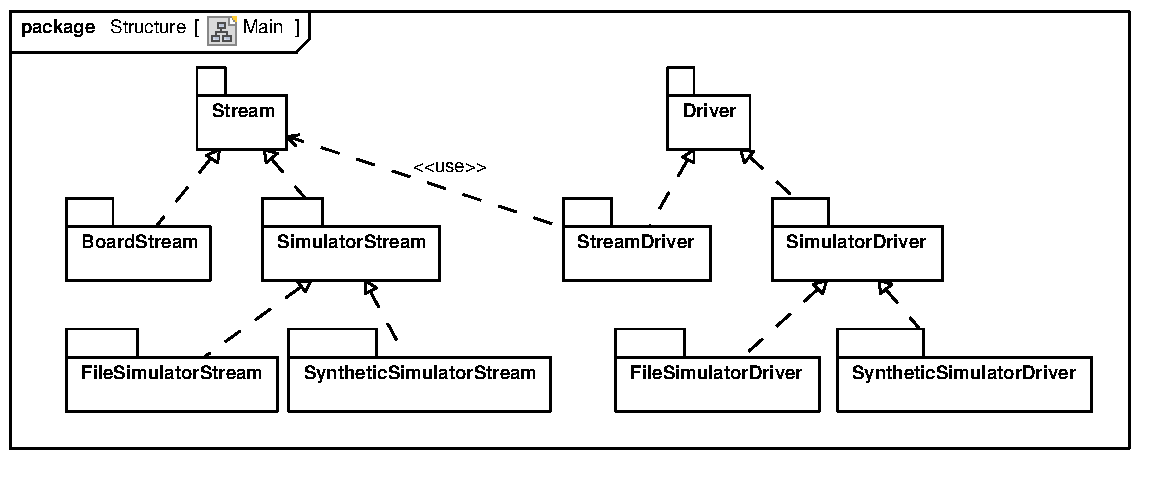
\includegraphics[scale=0.7]{UML_model/Class_Diagram__Structure__Main}
  \label{fig:class_diagram_main}
  \caption{Main packages class diagram.}
\end{figure}

% the test package structure
The test package structure, which is shown in Figure \ref{fig:class_diagram_test} reflects and mimics the code structure; the tests for an abstract package are abstract, and implemented by the package that tests a corresponding system implementation. 
This is a well known test pattern (the Abstract Test Pattern~\cite{Thomas2004}) used to test that the contracts defined in the abstractions are respected in the several implementations.  
For instance, package \lil{DriverT} contains abstract tests for the abstractions of package \lil{Driver}, package \lil{StreamDriverT} inherits the abstractions contained in \lil{DriverT} and makes them concrete, to test the corresponding implementation \lil{StreamDriver}; package \lil{StreamDriverT} also contains stand alone tests written specifically for the implementation contained in \lil{StreamDriver}.

\begin{figure}[htb!]
  \centering
  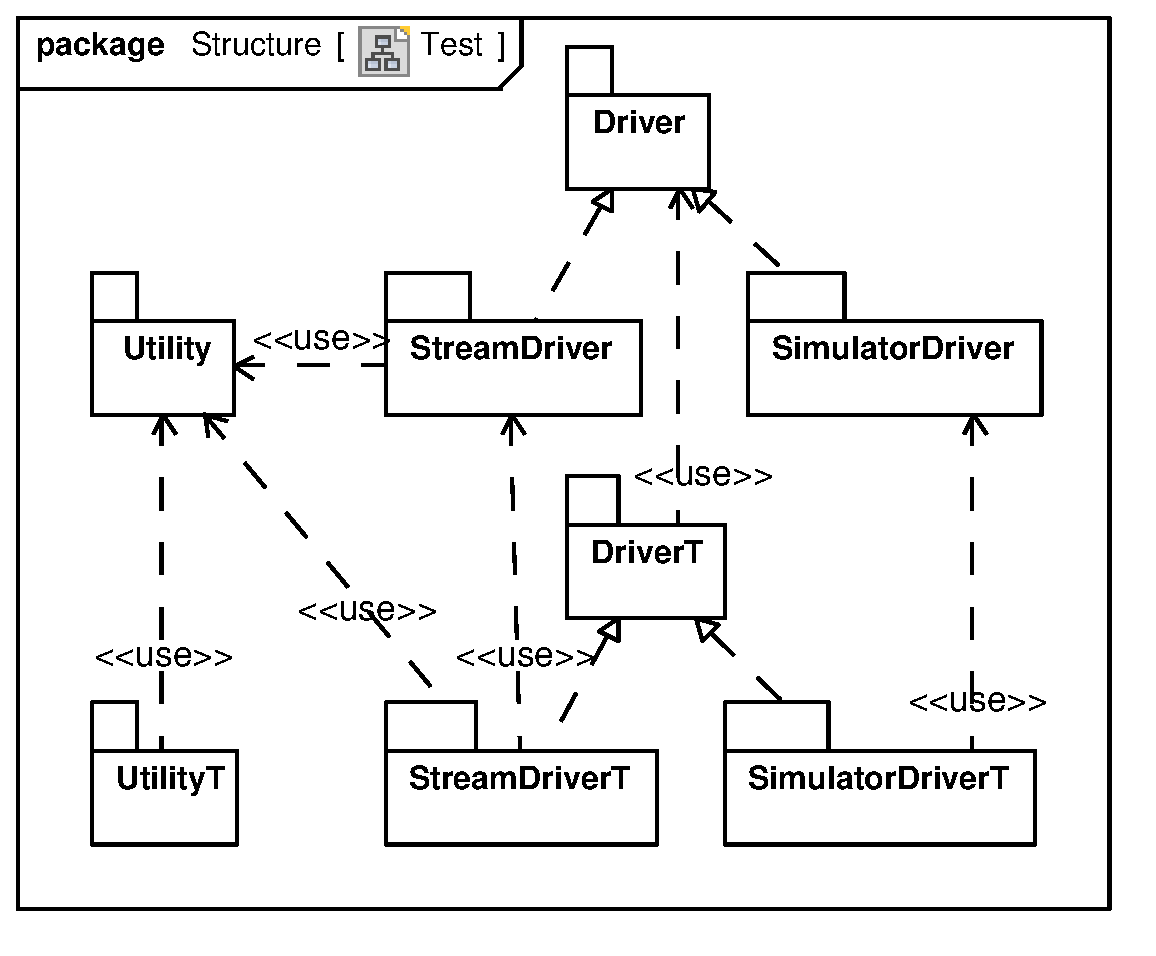
\includegraphics[scale=0.4]{UML_model/Class_Diagram__Structure__Test}
  \label{fig:class_diagram_test}
  \caption{Test packages class diagram.}
\end{figure}

\paragraph*{Generated tests}

% the generated test package structure
The JML specifications are used to generate tests.
The resulting test package structure is shown in Figure \ref{fig:class_diagram_generatedtest}.  
The package dependencies are defined by the specifications; for instance, \lil{SimulatorDriverST} are generated tests, they test (hence use) the implementation \lil{SimulatorDriver}, and have been generated using the corresponding specification \lil{SimulatorDriverS}.  
The generated tests do not maintain the inheritance structure of the code and the specification.

\begin{figure}[htb!]
  \centering
  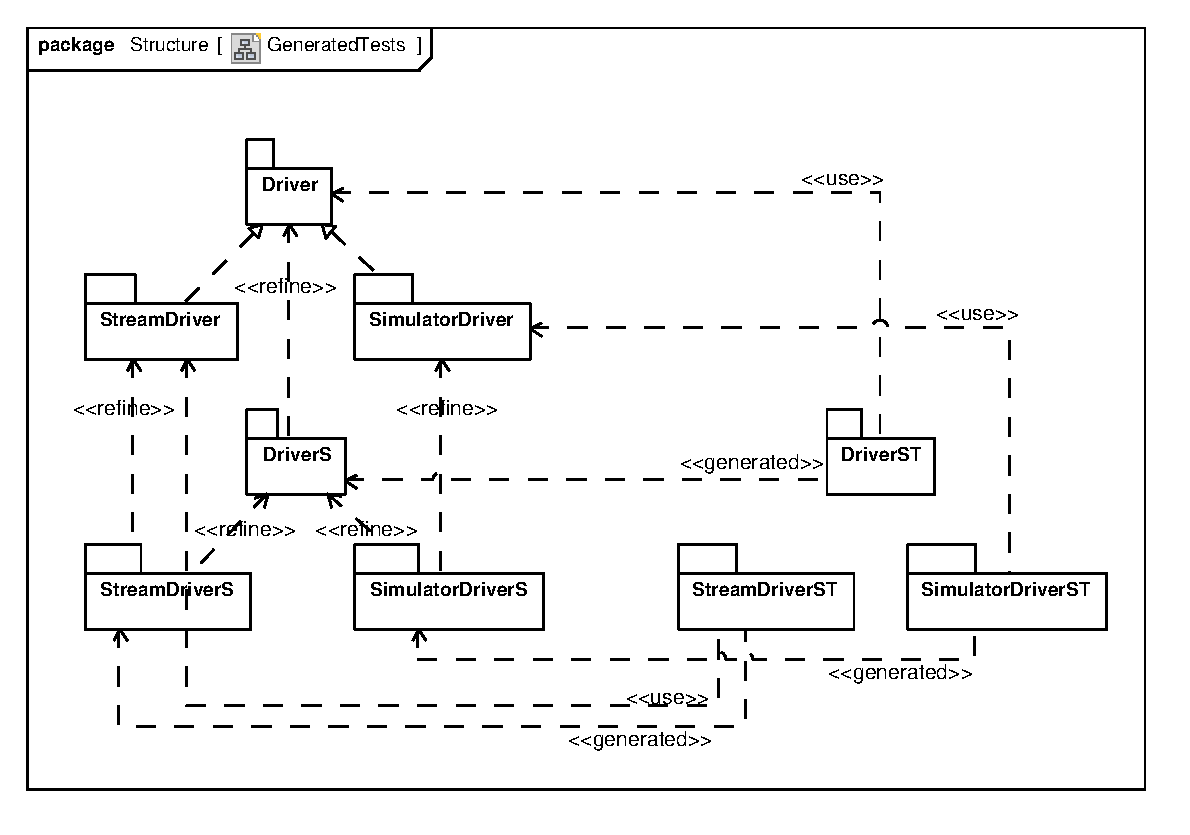
\includegraphics[scale=0.7]{UML_model/Class_Diagram__Structure__GeneratedTests}
  \label{fig:class_diagram_generatedtest}
  \caption{Generated test packages class diagram.}
\end{figure}

\paragraph*{On simulators, again}

% simulator roles in tests
The simulators are used in the hand made test suits as stubs.
The resulting structure is shown in Figure \ref{fig:class_diagram_streamdriver_test}.  
For instance, in Figure \ref{fig:class_diagram_streamdriver_test} the test suite \lil{StreamDriverT} is using the \lil{SimulatorStream} to properly simulate the \lil{Stream} used by \lil{StreamDriver}, which is the system under test.

\begin{figure}[htb!]
  \centering
  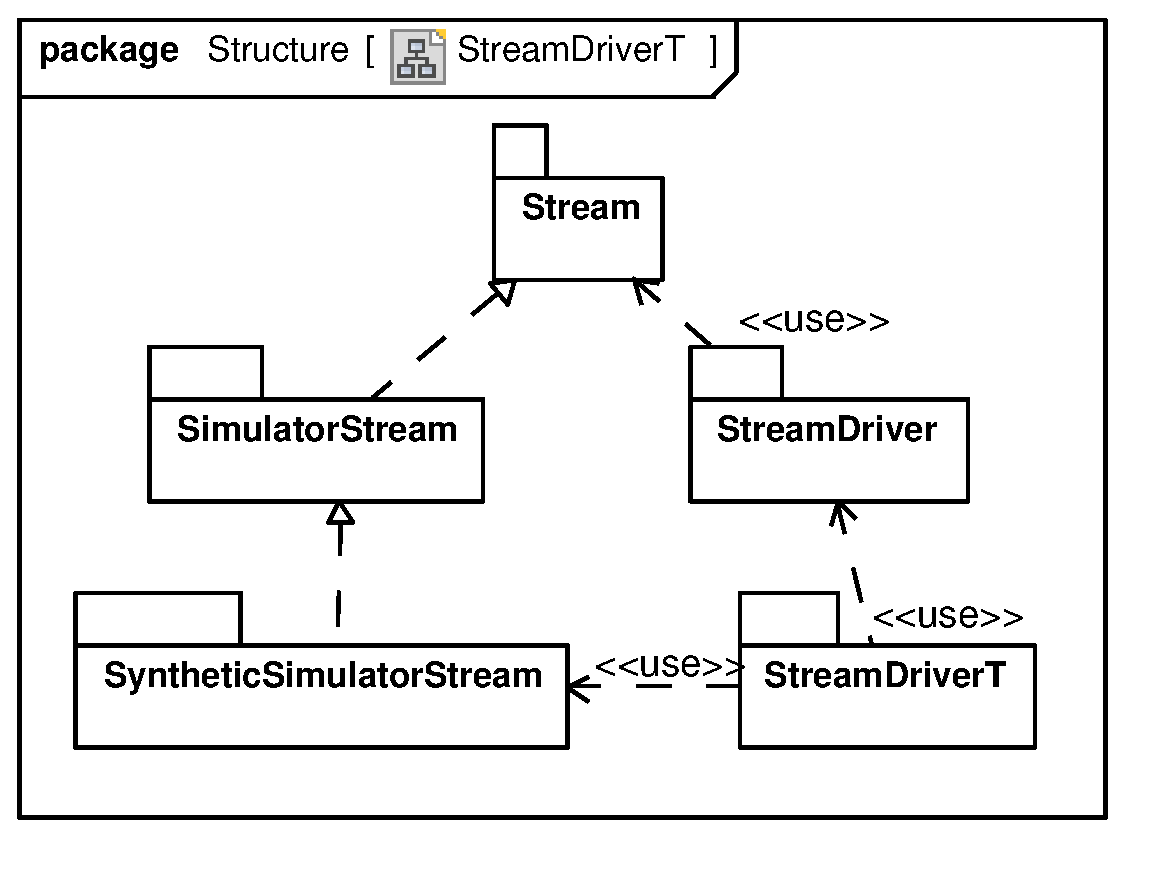
\includegraphics[scale=0.4]{UML_model/Class_Diagram__Structure__StreamDriverT}
  \label{fig:class_diagram_streamdriver_test}
  \caption{StreamDriver test packages class diagram: use of the stream
    simulator.}
\end{figure}

% simulator importance
The use of simulators to enable unit testing was essential to test the \STSB driver, since the physical board was not available.
The simulators are used in both the hand made and the generated test suite, since both need a proper set of stubs to be executed.



\subsection{Test cases on the job}
\label{subsec:test_cases_on_the_job}

% test suites sizes
The hand made test suite is composed by over 140 tests, while the generated one is 100 times bigger, totaling over 14000 tests.
The big number of generated tests can be understood looking closely at how the generated tests are created by the JML framework. 
The generated tests explore the possible input combinations on public methods, combining the type data ranges that are specified for the test suite (see \cite{Cheon-Leavens02} for more details on how the JML framework works on generating unit tests). 
For instance, let's suppose we want to test a method \lil{m(int p1, int p2)} for a class \lil{C}; the data ranges specified for type \lil{int} are \lil{\{1,2,3\}} and for type \lil{C} are the instances \lil{\{c1,c2,c3,c4\}}. 
The JML framework generates $24 = 3 \times 3 \times 4$ tests, since they are the combination of the data ranges involved (the data range of the parameters and the data range of the type owning the method under test). 
Neverteless, not all the generated tests are executed.
A generated test is not executed, unless the preconditions of the called method are satisfied. 
Thus, depending on the preconditions specified for a method, the number of the generated tests that are actually executed in the test suite can be significantly smaller compared to the total number of generated tests.

% test execution time, values
Test suites execution time are different, the hand made test suite, with the run time assertion checking active, runs completely in less than one minute on an average PC, while the generated test suite runs in more than 20 minutes (the rough ratio is $ 1 : 60 $). 
Most of the time is spent on setting up the suite, only considering the real execution of the tests, with no suite setup, the execution time reduces to less than 4 minutes (the rough ratio is $ 1 : 10 $).

% test effectiveness
Code coverage metrics is used to compare in a quantitative way the effectiveness of the test suites. 
This is only an indicator, since it is accepted that code coverage alone cannot asses the quality of a test suite\cite{Marick1999,Chockler2006}.
Various coverage metrics exist, the test suites are analyzed with statement code coverage (one of the simplest types)\footnote{The tool used to obtain statement code coverage metrics is \myhref{http://emma.sourceforge.net/}{Emma}.}: statement coverage reports whether each statement has been encountered during execution. 
Statement code coverage is easy to implement, but lacks the capability to explore the control flow graph associated to the code, that is,
decision branches are not explored. 
The coverage results are reported in the Table \ref{tab:statement_code_coverage}.

\begin{table}[htbp]
  \caption{Statement code coverage result, categorized by source package.}
  \label{tab:statement_code_coverage}
  \begin{center}
    \begin{tabular}{|c|c|c|c|}\hline
      & \textbf{\textit{hand}} & \textbf{\textit{generated}} &
      \textbf{\textit{total}} \\\hline
      \textbf{\textit{Driver}} & $15.9 \%$ & $6.3 \%$ & $15.9 \%$ \\\hline
      \textbf{\textit{StreamDriver}} & $76 \%$ & $79.7 \%$ & $88.5 \%$ \\\hline
      \textbf{\textit{SimulatorDriver}} & $64.9 \%$ & $44.2 \%$ &
      $71.2 \%$ \\\hline
      \textbf{\textit{Utility}} & $98.1 \%$ & $74.5 \%$ & $98.1 \%$ \\\hline
    \end{tabular}
  \end{center}
\end{table}



\subsection{Retrospective on test cases effectiveness}
\label{subsec:test_cases_retrospectives}

% <100 coverage measures, utility methods
The coverage measures reported in Table \ref{tab:statement_code_coverage} do not reach 100\%. 
This is because of two different effects: non public utility methods, and abstract methods in interfaces.
The effect of non public methods (package Java visibility) is that these methods are taken into account as public and protected ones are, during code coverage calculation; these methods are not part of the interface, they are not meant to be called by the system, and they are only used in object initialization or in object setups performed during unit tests. 
In fact there are package and private code blocks that are not reachable by construction from public and protected methods, and this is a precise characteristic reflecting the code architecture, meant to ease class instances setup and configuration for testing purposes. 
The used statement coverage tool cannot be configured to distinguish these code blocks, so this effect is unavoidable. 
The effect is mainly seen in low \lil{SimulatorDriver} code coverage figures: the \lil{SimulatorDriver} package has many utility non public methods.

% <100 coverage measures, interfaces
Regarding interfaces, an interface contains no statements, so when an interface method is called, it is the method of the implementation class used that is actually covered.
This effect is visible in \lil{Driver} coverage figures: \lil{Driver} package contains interfaces (that are not counted at all) and some very simple real class (exceptions) that are not throughly tested. 
The net result is extremely low statement code coverage figures because the very simple classes are the only ones that are actually covered. 

% code coverage interpretation
The statement code coverage figures show that the test suites do a good job on the most important package, the \lil{StreamDriver}. 
The generated test suite reaches almost $ 80 \% $, while the hand made tests have only a slightly lower coverage ratio: $ 76 \% $. 
The combination of test suites raise the coverage ratio to $ 88.5 \% $. 
This is a clear indication that one test suite is not completely overlapping the other: the intuition that test suites are not to be considered alternatives, but they need to be used together to achieve the higher benefits, is confirmed.
A similar indication is provided by \lil{SimulatorDriver} package as well.

% hand made unit test vs generated unit test
The qualitative difference of the two test suites can be understood observing how the suites are built. 
An hand made unit test usually requires objects initialization (it can involve several methods call), the call to the method under test, and the following assertions to verify the expected states change on the objects involved. 
A generated unit test has a more focused and limited scope: only one method call is performed in each test, it is difficult to explore complex behaviors. 
With a complete specification, and specifying large enough data ranges, the generated tests can achieve the same expressive power as the hand made ones; but the specification is not complete, and a large enough data ranges would take long to be developed.
The test suites give their best when used in a combined approach: the generated test suite, checking simpler and formalized behaviors, and the hand made, checking the more complex ones, whether formalized or not.  







% =====================================================================
\section{Related works}
\label{sec:related_works}

\todo{Out of scope: agile & formal used together, but not mixed}

\todo{describe and reference ``Agile Formal Method Engineering.'', formal centric}

\todo{describe and reference ``Formal Agility. How much of each?'', formal centric}

\todo{Mixin with test substitution}



% =====================================================================
\section{Conclusions}
\label{sec:conclusions}








\section{Extracts}

\paragraph*{limited resources}

% effect of the limited resources on the formal specifications
Hard constraints on driver delivery deadlines define the completeness level of the (\emph{just good enough}) specification.  
In \STSB driver JML specifies very simple behaviors (method oriented) on the whole driver implementation, and more complex behavior on the driver core interfaces.  
The software system parts not specified by the JML2 specification were specified using hand made unit tests.

\paragraph*{hand made unit tests}

% hand made unit tests purposes
Hand made unit tests specifies the behavior not specified by formal specification; nevertheless this is not the only purpose they have.
Hand made unit tests have been used to drive the development, since the Test Driven Development approach\cite{beck2003test} has been
followed during development.

% hand made unit tests suite structure
The hand made test suite primarily focuses on small features and use cases fragments that the system must implement, or for which an exceptional case has been specified. 
A test case is to be considered a rough specification written in imperative style. 
The common structure requires the objects initialization, followed by a sequence of method calls taking the objects into desired initial states; than the method under test is called and the objects states are finally inspected and verified. 
Mock objects can be used to limit module dependencies. 
The test suite should be composed only by unit tests, but usually some tests are more complex to be called proper unit tests; they can be seen as simple integration tests.


\paragraph{formal specification of the protocol}

% why a state machine has not been used to formally specify the protocol
\ST stream communication protocol is characterized by a well definite packet structure, and a well definite semantic on the packet contents.  
On the other hand, in the protocol, there are no strong constraints on synchronization, since the communication channel is splitted in two (in and out) separate concurrent and asynchronous channels.
The lack of hard synchronization constraints reduces the advantage to use a classical state machine based specification (as the one presented in \cite{Hubbers2004}), hence this option has been discarded during development.

\paragraph{jml}

% how jml generated tests work
The test suite generated is a collection of fine grained unit tests.
For each public method a set of tests is generated.
The specified behavior of the method is checked using the JML2 run time assertion checker, hence, an oracle is not needed.  
The generated tests send messages to the method under test, once the initial precondition check is passed (if it is not passed, the test is discarded), the test catch assertion violation exceptions; if a precondition is not met the test is not run, if the precondition is met the test is run and if the postcondition is not met an exception is fired and the test fails.
The test data used to build the tests is the only part that is required to be provided by the user.

\paragraph{unit tests}

% how unit tests should work
A proper stub, driver and oracle need to be identified for each method under test to obtain a proper unit test suite; stub, driver and oracle are the usual components found in the harness that enable test execution\cite{Binder1999}.  

% what is needed to test a package
To properly unit test a package, the following components need to be identified:
\begin{description}
\item[Stub or Skeleton]: a piece of code that simulates the activity of the modules that are not under tests.
\item[Driver]: a piece of code that calls in a proper way the module under test.
\item[Oracle]: a mechanism used for determining whether a test has passed or failed, comparing the output of the module under test to the output the oracle determines the module should have.
\end{description}

% junit
In JUnit\footnote{\myhref{http://www.junit.org/}{JUnit}}, which is the framework used to manage the implementation and execution of hand made and generated unit tests, there is no clear distinction between drivers, stubs, and oracles; none-less, even if a proper distinction
is not imposed by the framework, the conceptual distinction still holds.

% who provides what: hand made vs generated
Hand made unit tests and JML generated tests differ in how test components are provided.
The distinctions and similarities are summarized in Table \ref{tab:test_harness}.
\begin{table}[htbp]
  \caption{Hand made and generated tests harness.}
  \label{tab:test_harness}
  \begin{center}
    \begin{tabular}{|l|l|l|}\hline
      & \textbf{\textit{hand made}} & \textbf{\textit{JML}} \\\hline
      \textbf{\textit{Stub}} & to be provided & to be provided\\\hline
      \textbf{\textit{Driver}} & to be provided & automatic: 1 call\\\hline
      \textbf{\textit{Oracle}} & to be provided & 
      automatic: runtime assertion checker\\\hline
    \end{tabular}
  \end{center}
\end{table}

\todo{expand, test + RAC variations}

% test execution time, reasons
The execution time of the generated tests is influenced by:
\begin{itemize}
\item The number of the generated tests. 
This problem is not directly addressable, since it is the heart of the test suite generation creation method itself. 
All the combinations of possible inputs for each method under test must be generated.
\item The runtime assertion checker overhead. 
Each test is executed while RAC checks all the relevant properties. 
We can speculate that if the RAC assertions could be triggered on and off on single properties in a dynamic way (during runtime), a test suite would take advantage of this possibility, turning on the RAC only on the properties that have to be verified for the classes or methods under tests (and not for all the involved classes and methods); this could save time during the test suite execution.
\end{itemize}

% tests are helful
The generated test suite has been helpful to test the incrementally growing specifications and the finer details of each method, while the hand made one was helpful to verify the behavior of complex methods calls on objects initialized to specific states. 

% tests leads to a better design
An hand made test suite force the code to be test oriented, which usually leads to a better quality and more modularized source code\cite{Binder1999}.

\paragraph*{simulators and tests}

% simulators and tests
Simulators can be used to ease the tasks of developing the test harness components (Stub, Driver, Oracle).
A simulator can be used as a stub, to replace a module needed by the module under test.
A simulator can be used as a driver, stimulating the module under test.
Finally, a simulator can be used as an oracle, simulating the module under test.

% multiple simulators approach
The multiple simulators approach is not new, since it has been often used in embedded systems software testing\cite{Broekman2002}.  
This is a general approach that can (and should) be used to verify both the simulators built and the real systems.  
It can be easily implemented only if the code has been structured following the dependency inversion principle\cite{Martin1996} (see Figure
\ref{fig:class_diagram_main}).

\paragraph*{prototype history}

% tests and the first prototype, board side
The first \STSB prototype was meant to build empty packets, but the packets were built in a way not consistent with the specification.  
The board errors have been detected by simply using the driver implementation, the \lil{StreamDriver} package.

% tests and the second prototype, driver side
The second prototype was meant to build packets with values taken from real sensors installed on the board.  
The only sensors that were not yet working were the sensors devoted to the fast rate data streams (audio sensors).  
One error needed to be corrected in the driver implementation, because of a (rare) combinations of conditions that were not covered by the test cases, but that occasionally showed up during real use.
One error have been discovered in the low level system driver that the developed driver is using (the system driver is outside our development scope); to eliminate the error an upgrade of the low level driver to a new unreleased version were necessary. 
No other errors were detected on the driver side.

% tests and the second prototype, board side
The second prototype respected the packet byte structure specification, but was not fully compliant to the packet info structure specification and the single packet rules.
The formal JML specifications and the run time assertion checker enables the detection of these errors.
4 protocol errors regarding the packet info structure specification, and 2 protocol errors regarding the single packet rules were found. 
No other errors, except the mentioned ones, have been discovered.

\paragraph*{future work}

% problem on highest levels of the protocol
The highest levels of the protocol could be problematic (see \ref{subsec:data_stream_and_protocol_description}: ``Packet sequence rules'' and ``Packet input output asynchronous rules''). 
On these levels, the protocol properties regard sequences of packets, and testing them can be tricky, since the sequences of packets are not referred to explicitly, in the implementation.  

% solutions on highest levels of the protocol
Two possible strategies could be used:
\begin{itemize}
\item Translate the packet sequence properties in local packet properties (when possible).  
The advantage is to have properties shown as the usual pre-conditions, post-conditions and invariants.  
However, the localized properties can be more complex and less intuitive and comprehensible than the original ones; finally, some of the global properties could be impossible to translate.
\item Use separate utility classes, meant to verify a sequence of packages.  
This approach is not clean, since it requires adding and using new classes, unneeded by the core implementation, to verify the protocol.  It has the advantage of keeping the properties that have to be verified mostly unchanged.
\end{itemize}





% old paper
\section{OLD, to be reused}

% =====================================================================



% =====================================================================
\section{Related works}

JML has been used previously to verify a communication protocol in
\cite{Hubbers2004}, but the protocol is a smart card protocol, and it
is well represented through state machines, which are then refined
into JML properties.  The approach is in waterfall style; than the
need to develop the protocol, the specification and the implementation
concurrently is not addressed.  No hand made or generated test suites
are used, the code is specified with JML assertions, refined by the
state machine specifications, and then checked statically with
ESC/Java2 static checker\cite{CokKiniry04} and at runtime with JML2
tools RAC\cite{BurdyEtal05-STTT}.

The JML-JUnit automatic test suite generation tool has not been widely
used or assessed. It is described by its own creators in
\cite{Cheon2002,Cheon2004,Cheon2005}; it has been used in
\cite{Oriat2004} and \cite{Cheon2005}, but only as a stand alone test
suite, and, more importantly, only against proof of concepts system,
it has never be proved against real complex systems.  A brief
assessment of the JML-JUnit tool has been made in \cite{Tan2004}, the
analysis is based on injecting random generated errors in the source
code, and then evaluating the ratio of the errors found by the test
suite: the results shows that the JML-JUnit tool is not effective
enough if used as a stand alone tool. No attempts on running or
evaluating the generated test suite alongside with an hand made test
suite are made.








\section{Next papers}

\paragraph*{TDS: Test Driven Specification}

Approach:
\begin{itemize}
\item more specification used together: formal and not formal
\item formal specification is not complete: it is just good
  ``enough'', static checkers unfortunately cannot be used, since the
  specification is partial
\item use runtime assertion checker for formal specifications, on
  tests
\item use generated tests for formal specifications
\end{itemize}

Who drives what:
\begin{itemize}
\item specification (jml - formal specification or unit test -
  examples fragments) driven development
\item test driven specification
\item formal specification is not complete: it is just good
  ``enough'', static checkers unfortunately cannot be used, since the
  specification is partial
\item use runtime assertion checker for formal specifications, on
  tests
\item use generated tests for formal specifications
\end{itemize}

Benefits:
\begin{itemize}
\item real agile approach
\item real formal approach
\item use best of both worlds, do not try to use only on of them
\end{itemize}

Case example: actual paper, modified to fit the new parts, especially
the test driven specification part.

\paragraph*{BON}

\todo{describe approach: high level informal specifications with BON,
  iterative refinements of code, to distill test cases and formal
  specification of the interfaces}




% ======================================================================
%% \nocite{ex1,ex2}
\bibliographystyle{latex8} \bibliography{extra,%
  abbrev,%
  ads,%
  category,%
  complexity,%
  hypertext,%
  icsr,%
  knowledge,%
  languages,%
  linguistics,%
  meta,%
  metrics,%
  misc,%
  modeling,%
  modeltheory,%
  reuse,%
  rewriting,%
  softeng,%
  specification,%
  ssr,%
  technology,%
  theory,%
  web,%
  upcoming,%
  upcoming_conferences,%
  conferences,%
  workshops,%
  verification,%
  escjava,%
  jml,%
  nijmegen}

% ======================================================================
% Fin

\end{document}



%%% Local Variables: 
%%% mode: latex
%%% eval: 
%%% TeX-master: t
%%% End: 














% =====================================================================
\section{Data stream and protocol description}
\label{sec:data_stream_and_protocol_description}

\STSB and \STPU communicates via an Universal Serial Bus (USB)
interface.  A proprietary protocol is used on top of the USB serial
channels, the protocol is specified by
FTDI\footnote{\myhref{http://www.ftdichip.com/}{FTDI web site}}; FTDI
is the manufacturer of the USB controller chip used in the \STSB, the
FT2232H\cite{ftdi_ft232h_2009}.

The proprietary protocol enables the control and management of some of
the functionalities in FT232H chip (such as internal EEPROM read and
write, reset of the chip, etc.), as well as the definition of the
communication protocol and properties to be used in the asynchronous
channels (input and output channels) provided by FT232H.  These
functionalities are accessed via an Application Program Interface, the
API is provided by a driver developed directly by FTDI, which is
available for various systems (Linux 32 and 64 bits, Mac OS, Windows)
\cite{ftdi_d2xx_api_2009}.

Finally, a custom protocol has been developed to manage the entire
\STSB, built on top of the serial channels provided by the API.  The
custom protocol is meant to be used to read sensor data observations,
enable or disable sensors, configure on-board components (as the
Field-Programmable Gate Array and the micro processor); the protocol
main function is to read sensor data.

The protocol is asynchronous and packet based, the packets have a
fixed length.  The protocol has been divided in multiple layers to
ease its formal description.  The rationale is the following: mixing
up different abstraction levels of a protocol description can lead to
overly complex and unmanageable descriptions, especially when dealing
with formal ones.  The layers identified in protocol are the
following:

\begin{description}
\item[Packet byte structure]: the internal representation of the
  packet.
\item[Packet info structure]: the meaningful fields contained in the
  packets.
\item[Single packet rules]: the content acceptable values, and how
  they influence each other.
\item[Packet sequence rules]: the content acceptable values, based on
  values of previously received packets.
\item[Packet input output asynchronous rules]: the content acceptable
  values and reaction constraints on output packets, based on
  previously transmitted input packets.
\end{description}

We will examine the output sensor data packet, since it is the most
used and interesting one; we won't describe input or other output
packets.  We will examine the first three layers, that is: the packet
byte structure, the packet info structure and the single packet rules.

The packet byte and info structures of the output sensor data packet
reflect the board capabilities and built in sensors.  Essentially a
single packet has to accommodate various types of data:

\begin{itemize}
\item Fast data rate streams: audio data, 48KHz (standard audio) or
  96KHz (ultra audio).
\item Medium data rate streams: 5KHz.
\item Slow data rate streams: temperature, pression, accelerometer,
  etc.; all these sensor have a data rate lower than 5 KHz.
\item Metadatas: metadatas on sensors and board state.
\end{itemize}

The internal structure of the package (as we will see) is strictly
fixed, even if the data streams have different data rates.  This
choice originates from a trade-off between two constraints: the
efficiency of the transmission (redundant data to be minimized) and
the complexity to build a package (complexity to be minimized).  The
complexity minimization constraint rationale is the following: the
FPGA on the \STSB builds the packet, but the FPGA is also to be used
for various other specific tasks; it is important to maintain the
building packet code on the FPGA as simple and short as possible, to
leave enough space to implement other tasks.  The Output sensor data
packet structure is shown in Table \ref{tab:data_packet_structure},
the packet total length is 1024 bytes (512 16 bit words).

\begin{table}[htbp]
  \caption{Output sensor data packet structure.}
  \label{tab:data_packet_structure}
  \begin{center}
    \begin{tabular}{|c|l|}\hline
      \textbf{\textit{index}} & \textbf{\textit{function}}\\\hline
      0-1 & sentinel\\\hline
      2-7 & slow data\\\hline
      8-11 & metadata: board state\\\hline
      12-13 & reserved\\\hline
      14-15 & metadata: board state\\\hline
      16 & reserved\\\hline
      17-22 & frame 1\\\hline
      \ldots & \ldots\\\hline
      503-508 & frame 82\\\hline
    \end{tabular}
  \end{center}
\end{table}

The frames accommodate data from the fast and medium data rate streams
(there are 4 fast data rate stream and 8 medium data rate stream
channels).  There are 82 frames in a packet.  The frame structure is
shown in Table \ref{tab:frame_structure}.

\begin{table}[htbp]
  \caption{Output sensor data packet frame structure.}
  \label{tab:frame_structure}
  \begin{center}
    \begin{tabular}{|c|l|}\hline
      \textbf{\textit{index}} & \textbf{\textit{function}}\\\hline
      0 & metadata: frame description\\\hline
      1 & medium data rate data sample\\\hline
      2-5 & fast data rate data samples\\\hline
    \end{tabular}
  \end{center}
\end{table}

Looking at the structure described and the data rates frequencies, it
can be seen that there must be some subtle rule, to make all the
figures to add up; that is, to be capable to accommodate three
different rates outputs in a fixed structure, fixed length packet.
The subtleties lies in two forms of redundancies, for slow and medium
data rates:

\begin{itemize}
\item Slow data rates: slow data can be found at the beginning of each
  packet, the data is simply repeated (that is, it is equal to the
  previous packet in the stream) when no new data is available.
\item Medium data rates: the 8 medium rate channels are multiplexed
  together into the medium data rate data sample of each frame.  The
  medium data rate sample channel is a piece of info to be extracted
  from the frame description. Besides, the medium data rate data
  sample could contain no data at all, this information is to be
  extracted from the frame description. So, one frame could contain a
  medium data rate sample from channel 0, the following frame a sample
  from channel 5, the following frame no sample at all, etc.
\end{itemize}

The single packet rules delimit the boundaries of the values
obtainable from the packet: each defined sensor represented in the
packet, as well as the metadata describing the \STSB and the packet
and frame contents, are constrained by a range of acceptable values.
There are also rules affecting more than one value, these are
essentially validity rules (i.e. if a specific sensor is active the
reading value has to be in a defined range), and rules specifying a
correct sequence of frames (i.e. there can be only one switch in
sampling rate in the frame sequence of a single packet).



